\documentclass{article}
\usepackage{amsmath}
\usepackage{mathtools}
\usepackage{gensymb}
\usepackage[a4paper,inner=1.5cm,outer=1.5cm,top=2cm,bottom=0.5cm]{geometry} 
\usepackage{xcolor}                    
\usepackage{tikz}                           
\usepackage{multicol}
\usepackage{pgfplots}
\usetikzlibrary{calc}
\usetikzlibrary{intersections}
\usetikzlibrary{intersections,calc,angles,quotes}
\usetikzlibrary{shapes,arrows,positioning,decorations.pathreplacing,calc}
\usetikzlibrary{calc,angles,positioning,intersections,quotes,decorations.markings}
\usepackage{tkz-euclide}
\usetikzlibrary{backgrounds}
\usetikzlibrary{calc,through}
\usetikzlibrary{angles}
\usetikzlibrary{fadings}
\usetikzlibrary{shapes.geometric}
\usetikzlibrary{shapes.symbols}
\usepackage{draftwatermark}
\usepackage{mathptmx}

\SetWatermarkText{\textcolor{black!30}{Mathema Shukur}}
\SetWatermarkFontSize{2 cm}
\usepackage[utf8]{inputenc}
\usepackage{fontspec}

\setmainfont{[Kalpurush.ttf]}
\newfontface{\en}{[Arial.ttf]} %%this is optional, if you want to use a secondary font. Any english font is supported
\newlength\Radius
\setlength\Radius{4cm}
\begin{document} 
	\Large
	\textcolor{red}{Welcome To} 
	\\
	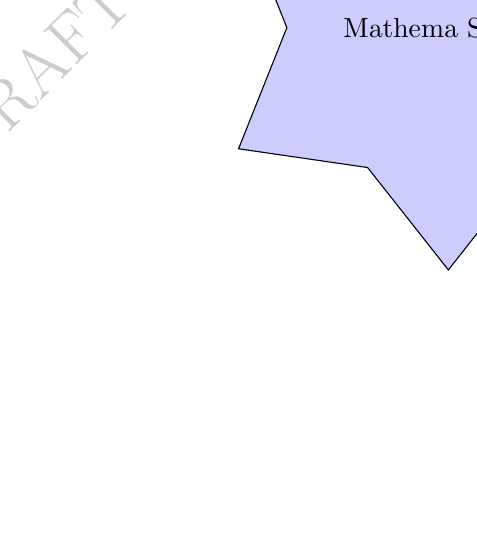
\begin{tikzpicture}
		\tikz \node [fill=blue!20,star,star points=6,draw] {Mathema Shukur };
	\end{tikzpicture}
	\\
	যাদের জন্যে প্রযোজ্যঃ  	\textcolor{magenta}{একাদশ ও দ্বাদশ শ্রেণীর শিক্ষার্থী} \\
	বিষয়ঃ \textcolor{magenta}{উচ্চতর গণিত ১ম পত্র} \\
	অধ্যায়ঃ \textcolor{magenta}{৩-সরলরেখা}\\ 
	Subtopicঃ  \textcolor{magenta}{ ক্ষেত্রফল শূন্য হলে ত্রিভুজে কী পরিবর্তন হয় ?  }\\
	\\
	 কোনো ত্রিভুজের শীর্ষ বিন্দু $(2,1)$, $(5,-1)$, $(8,-3)$ হলে এর ক্ষেত্রফল নির্ণয় কর \\
	 \\ 
	 $(x_1,y_1)=(2,1)$,\quad $(x_2,y_2)=(5,-1)$,\quad $(x_3,y_3)=(8,-3)$\\
	 \\ 
	 \begin{align*}
	 	\triangle ABC=	&\frac{1}{2}\begin{vmatrix}
	 		x_1 &	y_1 & 1\\
	 		x_2 & y_2 & 1\\
	 		x_3 & y_3 & 1
	 	\end{vmatrix}\\
	 	&=\frac{1}{2}\begin{vmatrix}
	 		2 & 1 & 1\\
	 		5 & -1 & 1\\
	 		8 & -3 & 1
	 	\end{vmatrix}\\
	 	&\boxed{Expansion \quad by \quad  First \quad  Column}\\ 
	 	&=\frac{1}{2}\left\{(2)\begin{vmatrix}
	 		-1 & 1\\
	 		-3 & 1
	 	\end{vmatrix}-(5)\begin{vmatrix}
	 		1 & 1\\
	 		-3 & 1
	 	\end{vmatrix}+(8)\begin{vmatrix}
	 		1 & 1\\
	 		-1 & 1
	 	\end{vmatrix}\right\}\\
	 	&=\frac{1}{2}\left[(2)(-1+3)-(5)(1+3)+(8)(1+1)\right]\\
	 	\\
	 	&=\frac{1}{2}\left[4-20+16\right]\\
	 	\\
	 	\triangle ABC	&=0
	 \end{align*}
 \\
 	\begin{tikzpicture}[transform shape,scale=1]
 	\draw [-latex,thick](-1,0) -- (10,0) node[right] {$x$} coordinate(x axis);
 	\draw [-latex,thick](0,-5) -- (0,3) node[above] {$y$} coordinate(y axis);
 	\fill[black] (0,0) circle (1.5 mm);
 	\node at (-0.3,-0.3) {$\textcolor{purple}{O}$};	
 	\fill[red] (2,1) circle (1 mm);
 	\fill[red] (5,-1) circle (1 mm);
 	\fill[red] (8,-3) circle (1 mm);	
 	\draw[thick,magenta,dashed] (2,1)--(5,-1);
 	\draw[thick,magenta,dashed] (5,-1)--(8,-3);
 		\node at (3,1) {$\textcolor{red}{(2,1)}$};	
 	\node at (6,-1) {$\textcolor{red}{(5,-1)}$};
 	\node at (9,-3) {$\textcolor{red}{(8,-3)}$};	
 \end{tikzpicture}
\\
ক্ষেত্রফল শূন্য হলে বিন্দু গুলি  সমরেখ হবে\\
\\ 
	দিনাজপুর বোর্ড-২০১৪\\ 
 কোনো ত্রিভুজের শীর্ষ বিন্দু $(2,-1)$, $(a+1,a-3)$, $(a+2,a)$ হলে এর ক্ষেত্রফল নির্ণয় কর । $a$ এর মান কত হলে বিন্দুগুলি সমরেখ হবে ?\\
 \\
  $(x_1,y_1)=(2,-1)$,\quad $(x_2,y_2)=(a+1,a-3)$,\quad $(x_3,y_3)=(a+2,a)$\\
 \\ 
 \begin{align*}
 	\triangle ABC=	&\frac{1}{2}\begin{vmatrix}
 		x_1 &	y_1 & 1\\
 		x_2 & y_2 & 1\\
 		x_3 & y_3 & 1
 	\end{vmatrix}\\
 	&=\frac{1}{2}\begin{vmatrix}
 		2 & -1 & 1\\
 		a+1 & a-3 & 1\\
 		a+2 & a & 1
 	\end{vmatrix}\\
 	&\boxed{Expansion \quad by \quad  First \quad  Column}\\ 
 	&=\frac{1}{2}\left\{(2)\begin{vmatrix}
 		a-3 & 1\\
 		a & 1
 	\end{vmatrix}-(a+1)\begin{vmatrix}
 		-1 & 1\\
 		a & 1
 	\end{vmatrix}+(a+2)\begin{vmatrix}
 		-1 & 1\\
 		a-3 & 1
 	\end{vmatrix}\right\}\\
 	&=\frac{1}{2}\left[(2)(a-3-a)-(a+1)(-1-a)+(a+2)(-1-a+3)\right]\\
 	&=\frac{1}{2}\left[-6+(a+1)^2-(a+2)(a-2)\right]\\
 	\triangle ABC	&=\frac{1}{2}\left[-6+a^2+2a+1-a^2+4\right]\\
 		\triangle ABC	&=\frac{1}{2}\left[2a-1\right]\\
 \end{align*}
\\
বিন্দু গুলো সমরেখ হবে যদি ক্ষেত্রফল শূন্য হয় \\
\\
\begin{align*}
	\triangle ABC	&=0\\
	\\
	\frac{1}{2}\left[2a-1\right]&=0\\
	\\
	2a-1&=0\\
	\\
	a&=\frac{1}{2}
\end{align*}
 চট্রগ্রাম বোর্ড-২০১৪\\ 
  $a$ এর মান কত হলে $(a,2-2a)$, $(1-a,2a)$ এবং $(-4-a,6-2a)$  বিন্দু তিনটি একই সরলরেখায় অবস্থিত । \\
   $\frac{1}{2},\quad -1$\\
   \\ 
   চট্রগ্রাম বোর্ড-২০১৬\\ 
   একটি ত্রিভুজের শীর্ষ বিন্দুর স্থানাঙ্ক $(t+1,1)$, $(2t+1,3)$, $(2t+2,2t)$। ত্রিভুজটির ক্ষেত্রফল নির্ণয় কর । দেখাও যে, $t=2$ অথবা $t=-\frac{1}{2}$ হলে বিন্দুগুলি সমরেখ হবে । \\
   \\
   $\frac{1}{2}(2t^2-3t-2)$\\ 
   \\
     চট্রগ্রাম বোর্ড-২০১২\\ 
   $\triangle OPQ$ এর শীর্ষত্রয়  $(0,0)$,  $(a\cos \beta, -a\sin \beta)$,  $(a\sin \alpha, a\cos \alpha)$ হলে দেখাও যে  $\alpha =\beta $ এর জন্য ত্রিভুজটির ক্ষেত্রফল সবচেয়ে বড় হবে এবং সবচেয়ে বড় মানটি বের কর \\
   \\
     $(x_1,y_1)=(0,0)$,\quad $(x_2,y_2)=(a\cos \beta, -a\sin \beta)$,\quad $(x_3,y_3)=(a\sin \alpha, a\cos \alpha)$\\
   \\ 
   \begin{align*}
   	\triangle OPQ=	&\frac{1}{2}\begin{vmatrix}
   		x_1 &	y_1 & 1\\
   		x_2 & y_2 & 1\\
   		x_3 & y_3 & 1
   	\end{vmatrix}\\
   	\\
   	&=\frac{1}{2}\begin{vmatrix}
   		0 & 0 & 1\\
   	a\cos \beta & -a\sin \beta& 1\\
   	a\sin \alpha & a\cos \alpha & 1
   	\end{vmatrix}\\
   	&\boxed{Expansion \quad by \quad  First \quad  Row}\\ 
   	&=\frac{1}{2}\left\{(0)\begin{vmatrix}
   	  -a\sin \beta& 1\\
   	a\cos \alpha & 1
   	\end{vmatrix}-(0)\begin{vmatrix}
   	 	a\cos \beta& 1\\
   	a\sin \alpha & 1 
   	\end{vmatrix}+(1)\begin{vmatrix}
   	 	a\cos \beta & -a\sin \beta\\
   	a\sin \alpha & a\cos \alpha 
   	\end{vmatrix}\right\}\\
   	\\
   	&=\frac{1}{2}\left[a^2\,\,\cos \alpha \,\,\cos \beta + a^2\,\,\sin \alpha\,\,\sin \beta \right]\\
   	\\
   	&=\frac{a^2}{2}(\cos \alpha \,\,\cos \beta + \sin \alpha\,\,\sin \beta)\\
   	\\
   	\triangle OPQ	&=\frac{a^2}{2} \cos (\alpha-\beta)
   \end{align*}
\\
$\cos (\alpha-\beta)$ এর সর্বোচ্চ মান $1$\\
\\
$\cos (\alpha-\beta)=1$\\
\\
$\cos (\alpha-\beta)=\cos 0$  \\
\\
$\alpha-\beta= 0$  \\
\\
$\alpha=\beta$  \\
\\
ত্রিভুজ ক্ষেত্রটির সবচেয়ে বড় মান \\ 
\\
 $\frac{a^2}{2} \cos (\alpha-\beta)$\\
 \\
 $=\frac{a^2}{2} (1)$\\
 \\ 
   $=\frac{a^2}{2}$\\
\end{document}